\section{Introduction}

The inverse folding problem in RNA design addresses a fundamental computational challenge: determining which nucleotide sequence will reliably fold into a specified three-dimensional backbone structure \citep{tang2024survey,tan2025r3design}. This problem represents the cornerstone of rational RNA engineering \citep{wong2024deep}, enabling systematic design of functional molecules for gene regulation \citep{green2014toehold}, therapeutics \citep{yip2024therapeutic}, and synthetic biology applications \citep{pfeifer2023harnessing}.

{
\emph{Designability}—defined as the total number or density of sequences that fold into a specific target structure—is a critical property for functional RNA. Highly designable structures are easier to discover, more mutation-robust \citep{england2003naturalselectdesignablefold}, and tend to inhabit thermodynamically favorable \emph{designable basins} (regions in sequence space with a high density of valid solutions) \citep{designability_li_1996}. Optimizing geometry alone may reach thin, fragile ridges in sequence space; coupling geometry with ensemble stability biases search toward these robust basins \citep{schuster1994rna2dshape}.
}

Contemporary geometric neural networks have achieved significant progress on this task \citep{wu2023integration,wu2023hierarchical,liu2025sentences,patil2024towards}. Models such as gRNAde \citep{joshi2025grnade} utilize graph neural networks with geometric vector perceptrons to capture spatial relationships within RNA tertiary structures, delivering impressive sequence recovery performance across benchmark datasets. 
{ However, unlike proteins that maintain relatively stable native folds, RNA molecules exhibit inherent conformational flexibility that causes them to sample multiple competing structures in solution \citep{ganser2019roles, zadeh2011nucleic}.}

Current inverse folding methods \citep{Hou2025ridiffusion, wong2024deep}, when optimized for sequence similarity or a single structural proxy, often neglect \emph{designability} and thermodynamic stability, and therefore \emph{do not} consistently adopt the intended conformation under physiological conditions.

Prevailing evaluations emphasize geometric correspondence (e.g., TMscore \citep{zhang2004tmscore} and RMSD for global alignment, pLDDT \citep{jumper2021alphafold2} for local fidelity), but these alone provide limited insight into \emph{ensemble viability} and \emph{designability}. As a result, sequences can score well structurally yet occupy narrow, unstable basins that admit competing conformations in solution \citep{bernard2024rnadvisor}. This evaluation-centric limitation produces sequences that achieve excellent structural scores while exhibiting poor ensemble behavior, sampling multiple competing conformations, and failing to demonstrate practical utility in biological applications \citep{zhou2023rna}. From a design perspective, single-objective optimization cannot fully address the multifaceted challenges inherent to RNA structural stability, where geometric fidelity must be balanced against thermodynamic preferences and conformational robustness.

\begin{figure}[!t] 
    \centering 
    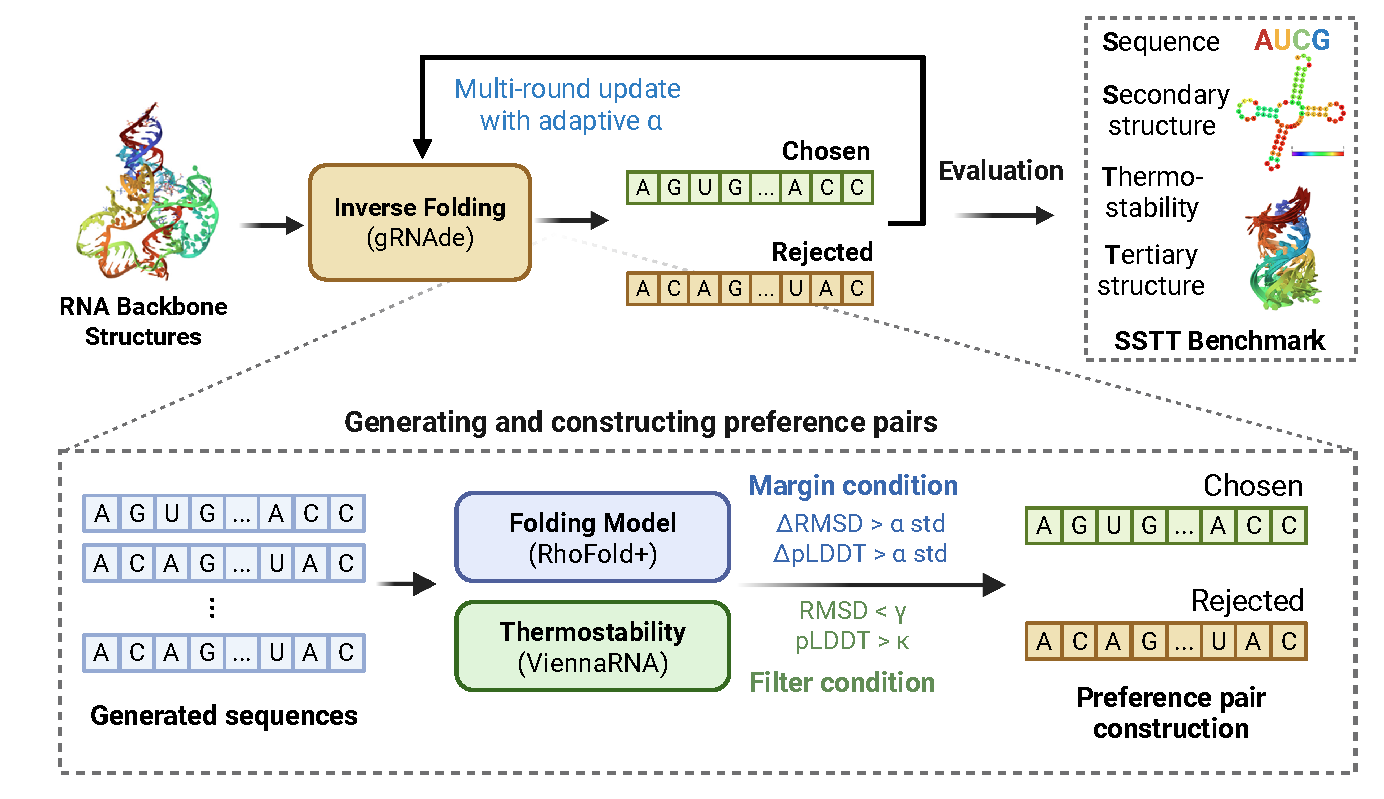
\includegraphics[width=0.9\textwidth]{figs/Main.pdf} 
    \vspace{-1em}
    \caption{Overview of RiboPO framework.} 
    \label{fig:main} 
\end{figure}

We present \textbf{RiboPO}, a preference-optimization framework for RNA tertiary inverse folding that addresses these limitations through two RNA-specific design choices: (i) preferences are constructed as $\varepsilon$-Pareto-dominance relations on standardized per-metric features, ensuring that recorded preferences correspond to candidates that improve \emph{simultaneously} on multiple noisy proxies; and (ii) the policy is trained with frozen-reference DPO under a decreasing-margin curriculum that we show is mirror descent on a KL-regularized trust region. Combined with an explicit structural quality gate that blocks compositional reward hacking via GC enrichment, these elements convert standard offline preference optimization into a stable RNA-design optimizer with provable drift bounds.

Our contributions are:
\begin{itemize}[leftmargin=*]
\item \textbf{Pareto-dominance preference learning under heteroscedastic physical proxies.} We construct preferences as $\varepsilon$-Pareto relations on per-metric standardized features (Section~\ref{subsubsec:pareto_pref}) with a confidence-thresholded margin $\alpha_r\!\cdot\!\sigma_m$ that we derive as a heteroscedastic Bradley--Terry confidence threshold (Appendix~\ref{app:hetero_derivation}). The resulting implicit reward is constrained to a Pareto-monotonic class --- the policy improves \emph{every} positive-weight scalarization simultaneously --- a guarantee strictly stronger than scalarized preference optimization.
\item \textbf{Trust-region multi-round optimization with off-policy bias bounds.} We prove that frozen-reference DPO with a decreasing-margin schedule has bounded cumulative KL drift (Theorem~\ref{thm:trust_region}) and that violating the frozen-reference assumption produces unbounded drift, matching the empirical ablation. We further bound the off-policy bias of static-pair multi-round DPO (Theorem~\ref{thm:off_policy}) and identify the empirical signature predicted by the bound: peak performance at intermediate rounds and gradual degradation when policy KL exceeds the candidate-pool entropy.
\item \textbf{Structural quality gate against RNA-specific reward hacking.} We identify GC enrichment as the dominant compositional failure mode of MFE-driven preference learning on RNA (sequence-structure degeneracy, Section~\ref{subsubsec:pareto_pref}) and show via a GC-controlled regression that $69\%$ of RiboPO's MFE improvement is GC-independent (Section~\ref{subsec:gc_control}). The structural quality gate $(\kappa,\gamma)=(0.70,8.0\,\text{\AA})$ is the load-bearing design choice that prevents the failure mode on weaker base models (e.g., RiFold) from propagating to the gRNAde main results.
\item \textbf{The SSTT evaluation suite.} We introduce SSTT (Sequence, Secondary, Tertiary, Thermostability), a comprehensive panel that simultaneously measures the four interdependent axes of RNA design quality. SSTT diagnostically catches reward-hacking failures that single-axis benchmarks miss, validated empirically by the Pareto-dominance ablation (Table~\ref{tab:ablation_multiround}) and the cross-architecture transfer to RiFold.
\end{itemize}

On the DAS benchmark (98 structures), RiboPO improves EternaFold scMCC by $+13\%$ ($p{=}1.2\!\times\!10^{-3}$ paired Wilcoxon), Vienna MFE by $-11.8\%$ ($p{=}7.0\!\times\!10^{-6}$), and target-structure probability by $+687\%$ ($p{=}1.6\!\times\!10^{-5}$). Under the joint structural-quality criterion (pLDDT$\geq$0.70 $\wedge$ RMSD$\leq$8\,\text{\AA}), RiboPO pass@1 ($0.258$) exceeds gRNAde pass@64 ($0.154$), a $64\times$ sample-efficiency gain. The framework transfers to RiFold (a stochastic-order autoregressive GNN) with the same loss and only learning-rate adaptation. Across 21 SSTT metrics, $20$ improve and $17$ are statistically significant; the only non-improver is sequence recovery, an explicit Pareto trade-off (INF for non-canonical contacts \emph{improves} by $+24\%$, indicating preserved functional contacts).
{ In Appendix~\ref{subsec:pareto} we show that these shifts correspond to movement into more \emph{designable basins} (lower energy, higher structural consistency).}
The ablation in Section~\ref{sec:experiments} confirms that each of the three design choices (variability-aware margin, frozen reference, structural quality gate) is individually load-bearing.